\documentclass[english,a4paper,oneside,9pt]{extarticle}
%\documentclass[english,a4paper,twoside,9pt]{extarticle}
% Author: 
%
%	Oliver Sheridan-Methven, November 2017.
%	
% Description:
%
%	A collection of extremely useful packages 
%	which have been accumulated over a long time,
%	all of which combine to make very nice LaTeX
%	documents. 



\usepackage{adjustbox} % Nice alternative to minipage.
\usepackage{afterpage} % To give the title page its own geometry.
\usepackage{amsmath} % Nice maths symbols.
\usepackage{amssymb} % Nice variable symbols.
\usepackage{array} % Allow for custom column widths in tables.
\usepackage{ltablex} % For long tables spanning multiple pages. % Must be before ARYDSHLN package!
\keepXColumns % Keeps the X column
\usepackage{arydshln} % Dashed lines using \hdashline \cdashline
\usepackage{bbm} % Gives Blackboard fonts.
\usepackage{blindtext} % Generates dummy maths. cf. lipsum.
\usepackage{calc} % Calculates widths of words. 
\usepackage{chngcntr} % Changing counters, e.g. with footnotes.
\usepackage[nostamp]{draftwatermark} % Gives a draft overlay. Use options [nostamp] or [final].
\usepackage{emptypage} % Empty pages have no headers and footers.
\usepackage{enumitem} % Nice listing options in itemize and enumerate.
\usepackage{esdiff} % Gives nice differential operators.
\usepackage{etoolbox} % For defining conditionals. 
\usepackage{fancyhdr} % Nice headers.
\usepackage{float} % Nice figure placement.
\usepackage[T1]{fontenc} % Nice range of text characters and accents.
\usepackage[bottom]{footmisc} % Nice footnote formatting.
\usepackage{graphicx} % Include figures.
\usepackage[notquote]{hanging} % For indenting later lines in a paragraph. USE the 'noquote' option else the `'` is overwritten, and breaks in maths mode!
\usepackage{ifoddpage} % Checks for odd or even page.
\usepackage[geometry]{ifsym} % Useful symbols.
\usepackage{imakeidx} % Makes the index.
\usepackage{indentfirst} % Indents the first paragraph.
\usepackage{letltxmacro} % For defining a nice SQRT symbol.
\usepackage{lipsum} % Useful for adding jargon.
\usepackage{listings} % The listings package for code.
\usepackage{marginnote} % For nice margin notes.
\usepackage{mathtools} % Gives the colon equals symbol.
\usepackage[framed,numbered,autolinebreaks,useliterate]{mcode} % Inports Listings package ideal for MATLAB.
\usepackage[framemethod=tikz]{mdframed} % Gives nices boxed and sidesrules.
\usepackage{multirow} % Nice table cells spanning many rows.
\usepackage{multicol} % If I want to use multiple columns.
\usepackage[numbers, sort&compress]{natbib} % Nice references.
\usepackage{sansmath} % Gives a changing math font. %% Must be before newpxtext/newpxmath ! %%
\usepackage{newpxtext} % Gives Palatino and Helvetica fonts.
\usepackage{newpxmath} % Gives Palatino and Helvetica fonts in maths. 
\usepackage{bm} % Bold math symbols. %% Needs to be loaded after newpxtext/math. %%
\usepackage{nicefrac} % Gives nice fractions for superscripts.
\usepackage{nomencl} % Gives a symbol nomenclature. 
\usepackage[super]{nth} % Gives nice ordinal superscripts, eg 1st, 2nd, etc.
\usepackage{parskip} % Gives nicer indenting.
\usepackage{physics} % Nice partial derivatives and BRAKET notation.
\usepackage{ragged2e} % For nice allignment.
%\usepackage[norefs]{refcheck} % Can show any unused references.
\usepackage{romannum} % Nice typing for roman numerals.
\usepackage{setspace} % Ideal for increasing line spacing. E.g.  \doublespacing
\usepackage{siunitx} % Nice formating of units.
\usepackage{sidenotes} % Nice margin figures and margin tables. 
\usepackage{subcaption} % Side by side figures.
\usepackage[textsize=small]{todonotes} % A nice TODO list. [disable] to supress.
\usepackage{tikz} % Nice diagrams.
\usepackage{titling} % Access title variables. 
\usepackage{titlesec} % Nice section title colouring options.
\usepackage[nottoc]{tocbibind} % Gives nices Table of Contents
\usepackage{xcolor} % This is useful for making greyed table cells, nice for headers. Known preamble placement issues.
\usepackage{xifthen}% Provides \isempty test.
\usepackage{xparse} % Gives \NewDocumentEnvironment which has nice optional argument handling.
\usepackage{xspace} % Gives nice spacing for commands.
%%%% Generally HYPERREF should be imported last. %%%%
\usepackage[colorlinks=true,linkcolor=black,urlcolor=black,citecolor=black,anchorcolor=black]{hyperref} % Colour links.
%%%% Should be loaded after hyperref. %%%%
\usepackage{cleveref} % Gives smart referencing. %% After Hyperref
\usepackage[margin=10pt,font=small, textfont=bf,labelfont=bf,labelsep=endash]{caption} % Caption figures and tables nicely. %% After cleveref.
\usepackage[left=60mm,right=26mm,top=30mm,bottom=29mm, heightrounded, marginparwidth=41mm, marginparsep=8mm, headsep=10mm]{geometry} % Use nice margins. Does give a small change in the default page margins. 

\makeatletter
\if@twoside % commands below work only for twoside option of \documentclass
\newgeometry{left=26mm,right=60mm,top=30mm,bottom=29mm, heightrounded, marginparwidth=41mm, marginparsep=8mm, headsep=10mm}
\fi
\makeatother

% Ensures subsubsections are numbered.
\setcounter{secnumdepth}{3}

% Making an index. 
\makeindex

% Making a nomenclature. 
\makenomenclature
% The column width for any nomenclature. 
\setlength\nomlabelwidth{0.2\linewidth}

% Set the table of content depth to only subsections. 
\setcounter{tocdepth}{2}

% Supressing bad box warnings
%\hbadness=10000 

% Where to search for figures. 
\graphicspath{{../../figures/}{../../figures/logos/}}

% Present the references in the order they are used.
\bibliographystyle{unsrtnat}
% Reduce spacing between references. 
\setlength{\bibsep}{0pt plus 0.3ex}

% Listing -> Code in environment labels.
\renewcommand{\lstlistingname}{Code}
\crefname{listing}{code}{codes}
\Crefname{listing}{Code}{Codes}
\lstset{
    numbers=left, 
    basicstyle=\ttfamily\footnotesize,
    frame=single, % adds a frame around the code
    xleftmargin=20.4pt,
    xrightmargin=3.4pt,
    %	numbersep=3mm,
}
\newfloat{lstfloat}{htbp}{lop} % environment for placing lisings in to make them float. 

% Nice paragraph indents.
\setlength{\parindent}{0mm}

% Giving the references the right title.
\renewcommand{\bibname}{References}
\renewcommand{\listfigurename}{List of figures}
\renewcommand{\listtablename}{List of tables}

% Removes most hyphenation.
\tolerance=1
\emergencystretch=\maxdimen
\hyphenpenalty=10000
\hbadness=10000

% To change the spacing in lists:
%\setlist{noitemsep} % or \setlist{noitemsep} to leave space around whole list
% or
\setenumerate{itemsep=-0.2em,topsep=0.5em} % Seems to look nice.

% Custom column widths using C{2cm}, L, R, etc.
\newcolumntype{L}[1]{>{\raggedright\let\newline\\\arraybackslash\hspace{0pt}}m{#1}}
\newcolumntype{C}[1]{>{\centering\let\newline\\\arraybackslash\hspace{0pt}}m{#1}}
\newcolumntype{R}[1]{>{\raggedleft\let\newline\\\arraybackslash\hspace{0pt}}m{#1}}

% Gives a nice column separation in multicolumn mode.
\setlength{\columnsep}{5mm}

% Figure environment for use in multicolumn. To put in captions use \captionof{figure}{content of caption}.
\newenvironment{Figure}
{\par\medskip\noindent\minipage{\linewidth}}
{\endminipage\par\medskip}

% Gives the nice SQRT symbol.
\makeatletter
\let\oldr@@t\r@@t
\def\r@@t#1#2{%
    \setbox0=\hbox{$\oldr@@t#1{#2\,}$}\dimen0=\ht0
    \advance\dimen0-0.2\ht0
    \setbox2=\hbox{\vrule height\ht0 depth -\dimen0}%
    {\box0\lower0.4pt\box2}}
\LetLtxMacro{\oldsqrt}{\sqrt}
\renewcommand*{\sqrt}[2][\ ]{\oldsqrt[#1]{#2}}
\makeatother

% Some common math operators which need their own typesetting.
\DeclareMathOperator{\sign}{sign}
\DeclareMathOperator*{\argmin}{argmin}
\DeclareMathOperator*{\argmax}{argmax}

% Number equations down to the subection level, e.g. 1.2.3 is the third equation in
% subsection 2 of section 1.
%\numberwithin{equation}{section}
\newcommand*\tageq{\refstepcounter{equation}\tag{\theequation}}

% This makes the footnote counter reset in each section.
\counterwithin*{footnote}{section}

% Nice spacing in the first row of a table
\newcommand{\firstrowspacing}{\rule{0pt}{2.6ex}}
% For a more open look in tables.
\setlength\extrarowheight{3pt} 

% Some useful text commands.
\newcommand{\nag}{NAG\textsuperscript{\textregistered}\xspace}
\newcommand{\arm}{Arm\textsuperscript{\textregistered}\xspace}

% For nice headers and footers.
\pagestyle{fancy}
\fancyhf{}
\renewcommand{\headrulewidth}{0pt}
\newlength{\oneinch}
\setlength\oneinch{1in}
\newlength{\innermarginonesided}

\newtoggle{TWOSIDED}
\togglefalse{TWOSIDED}
\makeatletter
\if@twoside % commands below work only for twoside option of \documentclass
\toggletrue{TWOSIDED}
\fi
\makeatother

\setlength\innermarginonesided{\paperwidth-\textwidth-\oddsidemargin-1in}
\makeatletter
\if@twoside
\setlength\innermarginonesided{\evensidemargin+1in}
\fi
\makeatother


\definecolor{header1}{RGB}{253,252,204}
\definecolor{header2}{RGB}{204,236,255}
\definecolor{header3}{RGB}{37,141,255}
\definecolor{header4}{RGB}{0,117,246}
\definecolor{header5}{RGB}{0,73,154}
\fancyhead[RE]{%
    \begin{adjustbox}{left, minipage=0.9\paperwidth}
        \hspace*{-0.8\innermarginonesided}
        \begin{tikzpicture}[overlay]
        \fill[fill=header5, draw=header5, minimum height=8mm, minimum width=16.4cm,anchor=west] (0,-1.4em) rectangle (1.0\linewidth,1.5em);
        \fill[fill=header4, draw=header4, minimum height=8mm, minimum width=16.4cm,anchor=west] (0.7\linewidth,-1.4em) rectangle (\linewidth,1.5em);
        \fill[fill=header3, draw=header3, minimum height=8mm, minimum width=16.4cm,anchor=west] (0.8\linewidth,-1.4em) rectangle (\linewidth,1.5em);
        \fill[fill=header2, draw=header2, minimum height=8mm, minimum width=16.4cm,anchor=west] (0.85\linewidth,-1.4em) rectangle (\linewidth,1.5em);        
        \fill[fill=header1, draw=header1, minimum height=8mm, minimum width=16.4cm,anchor=east] (0.9\linewidth,-1.4em) rectangle (\linewidth,1.5em);
        \end{tikzpicture}%
\end{adjustbox}%
    }
\fancyhead[LO]{%
    \begin{adjustbox}{right, minipage=0.9\paperwidth}
        \hspace*{0.8\innermarginonesided}
        \begin{tikzpicture}[overlay]
        \fill[fill=header5, draw=header5, minimum height=8mm, minimum width=16.4cm,anchor=east] (0,-1.4em) rectangle (1.0\linewidth,1.5em);
        \fill[fill=header4, draw=header4, minimum height=8mm, minimum width=16.4cm,anchor=east] (0,-1.4em) rectangle (0.3\linewidth,1.5em);
        \fill[fill=header3, draw=header3, minimum height=8mm, minimum width=16.4cm,anchor=east] (0,-1.4em) rectangle (0.2\linewidth,1.5em);
        \fill[fill=header2, draw=header2, minimum height=8mm, minimum width=16.4cm,anchor=east] (0,-1.4em) rectangle (0.15\linewidth,1.5em);        
        \fill[fill=header1, draw=header1, minimum height=8mm, minimum width=16.4cm,anchor=east] (0,-1.4em) rectangle (0.1\linewidth,1.5em);
        \end{tikzpicture}%
\end{adjustbox}%
    }

\newcommand{\textoverline}[1]{$\overline{\mbox{#1}}$}
% The footers are specified but are not the same margin widths as the headers. 
\fancyfoot[LE]{\hspace*{-0.8\innermarginonesided}\begin{adjustbox}{left, minipage=0.9\paperwidth}
        \raggedright
        \color{cyan}\textoverline{\color{black}\underline{\hphantom{\ }\thepage
                \begin{minipage}[c]{0\linewidth}
                    \rule{0pt}{2.5ex}
                \end{minipage}
                \rule{0.9\linewidth}{0pt}\rule{0pt}{2.0ex}}}
    \end{adjustbox}
}
\fancyfoot[RO]{\hspace*{0.8\innermarginonesided}\begin{adjustbox}{right, minipage=0.9\paperwidth}
        \raggedleft
        \color{cyan}\textoverline{\color{black}\underline{
                \begin{minipage}[c]{0\linewidth}
                    \rule{0pt}{2.5ex}
                \end{minipage}
                \rule{0.9\linewidth}{0pt}\rule{0pt}{2.0ex}\thepage\hphantom{\ }}}
    \end{adjustbox}
}
\fancypagestyle{plain}{%
    \fancyhf{}%
    \renewcommand*{\headrulewidth}{0pt}%
}
\cfoot{}


% Make margin notes small
\renewcommand*{\marginfont}{\noindent \small}
%\IfBooleanTF{@twoside}{\reversemarginpar}{}% If I want a wider margin by the binding.
% Ensuring nice justification.
\renewcommand\raggedrightmarginnote{\sloppy}
\renewcommand\raggedleftmarginnote{\sloppy}

% Gives a nice quote environment.
\NewDocumentEnvironment{myquote}{O{}}{%
    \begin{center}
        \begin{minipage}{0.85\linewidth}
            \vspace{1ex}
            \centering \itshape \justifying}
        {%
            \ifthenelse{\isempty{#1}}{}{
                \begin{flushright}%The author/source.
                    \normalfont #1
            \end{flushright}}
            \vspace{1ex}
        \end{minipage}
    \end{center}
}

% Gives a nice siderule environment. e.g. \begin{siderules}
\newmdenv[topline=false,bottomline=false,rightline=false,skipabove=\topsep,skipbelow=\topsep]{siderules}

% For a numbered description. Use inside enumerate, \litem{Something} etc. 
\newcommand\litem[1]{\item{\textbf{\underline{\smash{{#1}}:}}}}

% Nice spacing in lists
%\setlist{listparindent=\parindent,parsep=1ex} 

% This aligns figures in the adjust box environment to the inner margin. For use with "myalignedfigure" (below).
\newcommand{\aligninner}{\ifoddpage \raggedright \else \raggedleft \fi}%

% Gives a nice aligned figure environment, where figures are flush to the inner margin overflowing off the outer margin first. Useful for very wide figures, or set of lots of sub figures. 
\NewDocumentEnvironment{myalignedfigure}{O{1.3} O{htb}}{% fractional_linewidth,  position
    \begin{figure}[#2]
        \checkoddpage
        \edef\whichside{\ifoddpage left\else right\fi}
        \begin{adjustbox}{\whichside, minipage=#1\linewidth}}
        {%
        \end{adjustbox}
    \end{figure}
}

% Gives a nice draft text.
\SetWatermarkScale{1}
\SetWatermarkLightness{0.9}

% The oxford comma from cref for multiple citations. 
\newcommand{\creflastconjunction}{, and\nobreakspace}

% Define the dummy sentence, an ancient palindrome.
\def\sator{Sator Arepo tenet opera rotas.\xspace}

% A command to print the sentence repeatedly.
% Argument #1 is the number of times to repeat it.
\newcount\loopcounter
\def\dummysentences#1{%
    \loopcounter = #1
    \loop
    \sator\ %
    \advance\loopcounter by -1
    \ifnum\loopcounter > 0
    \repeat%
}

% Oxford blue
\definecolor{oxfordblue}{RGB}{0, 33, 71}

% Ensuring side boxes have shadows. 
\usetikzlibrary{shadows} % For shadowed boxes.
\tikzset{every shadow/.style={opacity=1}} % Shadows given full opacity. 

% Temporary environment for the InFoMM side bubble. 
\NewDocumentEnvironment{mysidenote}{}{% verticle offset
    \noindent
    \begin{minipage}[t]{\linewidth}		\begin{mdframed}[roundcorner=5pt, linecolor=oxfordblue, linewidth=2pt, backgroundcolor=yellow!40, shadow=true,shadowcolor=black,shadowsize=6pt]\raggedright
        }
        {
        \end{mdframed}
    \end{minipage}
}

% The final command for an InFoMM margin bubble. 
\newcommand{\infommmarginnote}[2][0mm]{\marginnote{\large\sffamily{}\sansmath\begin{mysidenote}{#2}\end{mysidenote}}[{#1}]}

% Useful for drawing a page border. 
\usetikzlibrary{calc}

% Enable blind maths. 
\blindmathtrue

%InFoMM glossary
\NewDocumentEnvironment{infommitemize}{}{% verticle offset
    \noindent
    \begin{itemize}[label={\color{cyan}{$\blacksquare$}}]
    }
    {%
    \end{itemize}
}

\newcommand{\coverimage}[1][cover_image]{
    \newcommand{\thecoverimage}{#1}
}

% Nice colouring of section titles
\titleformat{\section}
{\color{oxfordblue}\normalfont\fontsize{16}{20}\selectfont\bfseries}
{\color{oxfordblue}\thesection}{1em}{\thesection.\hspace{1ex}}
\titleformat{\subsection}
{\color{cyan}\normalfont\Large\bfseries}
{\color{cyan}\thesection}{1em}{}
\titleformat{\subsubsection}
{\color{cyan}\normalfont\Large\bfseries}
{\color{cyan}\thesection}{1em}{}

% Shorten the spacing after section headings
\titlespacing\section{0pt}{12pt plus 4pt minus 2pt}{0pt plus 2pt minus 2pt}
\titlespacing\subsection{0pt}{12pt plus 4pt minus 2pt}{0pt plus 2pt minus 2pt}
\titlespacing\subsubsection{0pt}{12pt plus 4pt minus 2pt}{0pt plus 2pt minus 2pt}



% Remove section numbers in TOC. 
%\makeatletter
%\let\latexl@section\l@section
%\def\l@section#1#2{\begingroup\let\numberline\@gobble\latexl@section{#1}{#2}\endgroup}
%\makeatother
% Remove subsection numbers in TOC. 
\makeatletter
\let\latexl@subsection\l@subsection
\def\l@subsection#1#2{\begingroup\let\numberline\@gobble\latexl@subsection{\quad#1}{#2}\endgroup}
\makeatother





\title{Long-term degradation \\ of lithium-ion batteries}
\author{Scott Marquis}
\coverimage[solar-and-wind-hybrid] % Specify your own image using [].
\companylogo[siemens-logo]

\usepackage{overpic}
\usepackage{booktabs}

\newcommand{\ts}[1]{_{\text{#1}}}
\newcommand{\Xav}[1]{\bar{#1}}
\newcommand{\YZav}[1]{\langle #1 \rangle}
\newcommand{\XYZav}[1]{\YZav{\Xav{#1}}}

\newcommand{\good}[1]{\textcolor{green}{#1}}
\newcommand{\ok}[1]{\textcolor{orange}{#1}}
\newcommand{\bad}[1]{\textcolor{red}{#1}}

\newcommand{\cmark}[1][green,fill=green]{\tikz[baseline=-0.5ex]\draw[#1,radius=3pt] (0,0) circle ;}%
\newcommand{\okmark}[1][orange,fill=orange]{\tikz[baseline=-0.5ex]\draw[#1,radius=3pt] (0,0) circle ;}%
\newcommand{\xmark}[1][red,fill=red]{\tikz[baseline=-0.5ex]\draw[#1,radius=3pt] (0,0) circle ;}%
\newcommand{\best}[1][green,fill=green]{\tikz[baseline=-0.5ex]\draw[#1,radius=3pt] (0,0) circle ;}%


\begin{document}

% The cover page is a designed to look best on A4 and is designed to be a
% "What you see is what you get".
\thispagestyle{empty} % 'gobble' pagestyle throws issues with nomencl package. 
\afterpage{
%\pagestyle{empty}
\newgeometry{left = 20mm, right = 20mm, top = 15mm, bottom = 10mm}

\newgeometry{left = 20mm, right = 20mm, top = 30mm, bottom = 30mm}
\pagestyle{empty}
\begin{tikzpicture}[remember picture, overlay]
\draw [line width=2mm, oxfordblue]
($ (current page.south west) + (8mm, 8mm) $)
rectangle
($ (current page.north east) + (-8mm, -8mm)$);
\node[anchor=north west, xshift=10mm, yshift=-10mm] at (current page.north west) {
\includegraphics[width=0.3\linewidth]{epsrc_logo}};
\node[anchor=north east, xshift=-10mm, yshift=-10mm] at (current page.north east) {
\includegraphics[width=0.3\linewidth]{infomm_logo_blue}};
\node[anchor=south west, xshift=10mm, yshift=10mm] at (current page.south west) {
\includegraphics[width=0.3\linewidth]{oxford_logo_blue_long}};
\node[anchor=south east, xshift=-10mm, yshift=10mm] at (current page.south east) {\includegraphics[width=0.4\linewidth]{\thecompanylogo}};
\end{tikzpicture}

\begin{center}
\vfill
{\fontsize{25}{28}\selectfont\color{oxfordblue}\textbf{EPSRC Centre for Doctoral Training in Industrially Focused Mathematical Modelling}}
\vfill
\begin{figure}[h]
\centering
\includegraphics[width=0.7\linewidth]{\thecoverimage}
\end{figure}
\vfill
{\fontsize{25}{28}\selectfont\color{oxfordblue}\textbf{\thetitle}}\\
\vfill
{\fontsize{20}{25}\selectfont\color{oxfordblue}\color{oxfordblue}\textbf{\theauthor}}
\vfill
\end{center}
\restoregeometry
}
\clearpage
	  % The widths and heights here might need a bit of fine tuning.
% Table of contents page.
\afterpage{
	\titleformat{\section}
	{\color{oxfordblue}\normalfont\fontsize{16}{20}\selectfont\bfseries}
	{\color{black}\thesection}{1em}{}
\pagestyle{empty}
\newgeometry{left=110mm,right=20mm,top=30mm,bottom=29mm, heightrounded, marginparwidth=100mm, marginparsep=5mm}
\reversemarginpar
\noindent
\doublespacing
\begin{minipage}[t]{\linewidth}
\tableofcontents
\end{minipage} \\
\marginpar{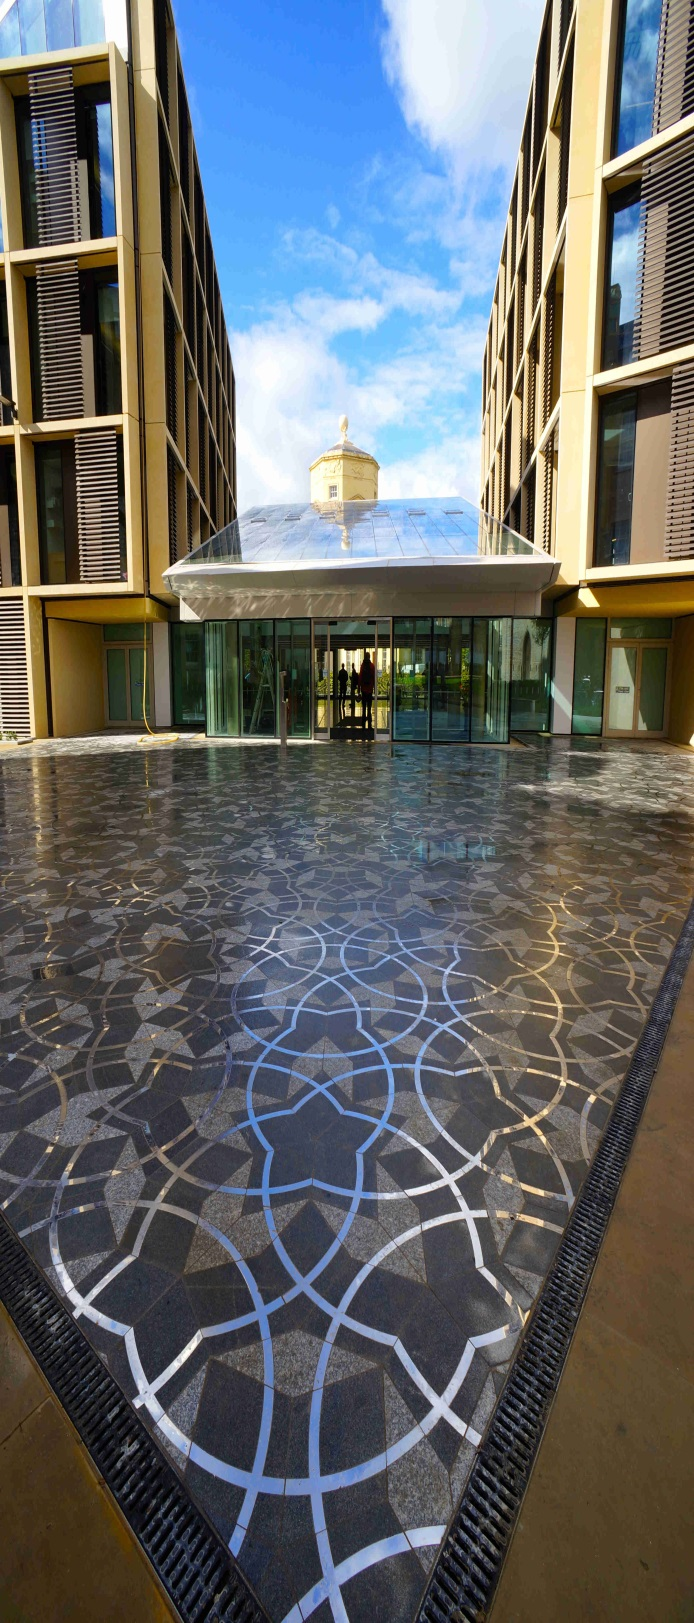
\includegraphics[width=\linewidth]{andrew_wiles_building}}
\clearpage
}

\cleardoublepage % Double page as page numbering starts at 1.
\setcounter{section}{0}
\pagenumbering{arabic}
 % Don't touch.

\section{Introduction}
\subsection{Background information}

With the shift to vehicle electrification and renewable energy sources, lithium-ion batteries are emerging as one of the most important technologies of the 21st century. Siemens utilise lithium-ion batteries in grid-scale energy storage systems, which correct for offsets in electricity supply and demand. This in turn makes intermittent energy sources such as solar and wind viable.

\infommmarginnote[-1cm]{The proper management of lithium-ion battery systems requires a quantitative understanding of degradation.}
To properly manage such large-scale battery systems, it is essential to understand cell \emph{degradation}. A quantitative description of degradation would allow for accurate forecasting of the value of the battery system. This would then facilitate the formation of strategies for optimal usage of the system.

\subsection{Lithium-ion pouch cells}
A common format of a lithium-ion battery is the pouch cell format, displayed in \Cref{fig:pouch-cell}. The interior of the cell consists of two electrically conducting porous electrodes separated by an electrically insulating porous separator. Each electrode consists of \emph{active material} particles, presented as circles in \Cref{fig:pouch-cell}, and a \emph{binder} material, which is not shown in \Cref{fig:pouch-cell}. Within the pores of the \emph{electrode} and \emph{separators}, an liquid \emph{electrolyte} is present. The two electrodes are sandwiched between two electrically conducting \emph{current collectors} which have tabs at the top to allow for an easy connection to an external circuit.

\infommmarginnote[2cm]{Lithium-ion batteries consits of two separated porous electrodes within an electrolyte.}
\begin{figure}[htbp]
	\centering
	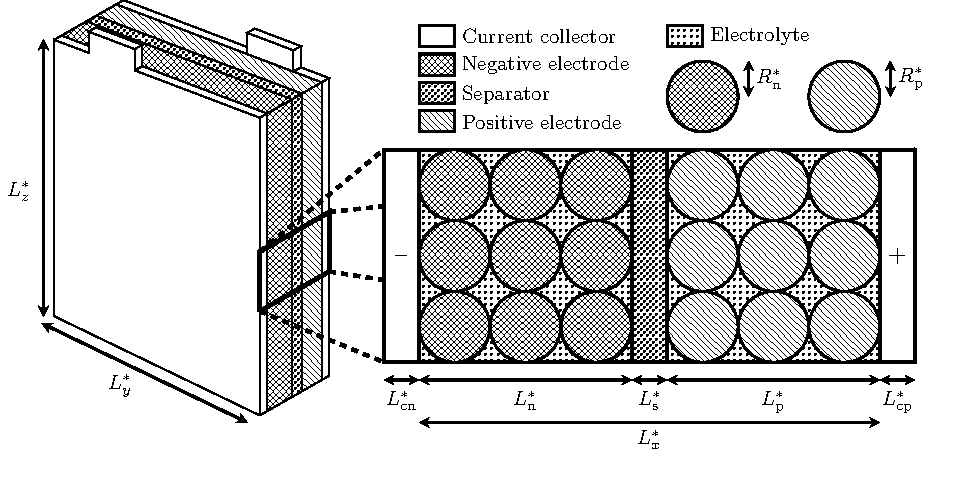
\includegraphics[width=\textwidth]{pouch-cell.pdf}
	\caption{Schematic of a lithium-ion pouch cell.}
	\label{fig:pouch-cell}
\end{figure}

When a lithium-ion cell is discharged by connecting the two tabs to an external circuit, lithium \emph{intercalated} in the active material of the negative electrode travels to the surface of the active material where an electrochemical reaction occurs. This reaction converts intercalated lithium into lithium ions contained in the electrolyte and electrons contained in the negative electrode. The lithium-ions then travel through the electrolyte to the surface of the positive active material particles where they recombine with an electron to form lithium intercalated in the positive active material. During charge, the process occurs in reverse, driven by an applied voltage.

\subsection{Solid--Electrolyte Interphase (SEI) Growth}
\infommmarginnote[-1.3em]{SEI growth is a key degradation mechanism.}
SEI growth is one of the dominate degradation mechanisms occurring within lithium-ion batteries. The SEI is a layer that forms on the surface of the negative active material particles as a result of the occurrence of parasitic side reactions. In \Cref{fig:sei}, we present a schematic of the structure of the SEI and the side reaction which creates new SEI. The SEI consists of two layers, a dense inner layer and a porous outer layer. In the creation of SEI, electrons within the negative electrode travel through the dense inner layer whilst lithium ions and \emph{solvent} molecules from the electrolyte travel through the pores of the outer SEI. These three species then combine through an electrochemical reaction at the surface of the inner and outer SEI to form fresh SEI. Since the growth of SEI consumes lithium ions, cyclable lithium is lost from the battery which results in capacity fade. In the presence of SEI, lithium ions can still intercalate into the negative active material. However, since they now have to travel through the inner SEI, there is increased resistance to this process. This results in increased internal resistances within the cell which make the cell less efficient.

\infommmarginnote[1.5cm]{The SEI consists of a dense inner layer and a porous outer layer and is formed through parasitic side reactions.}
\begin{figure}[htbp]
	\centering
	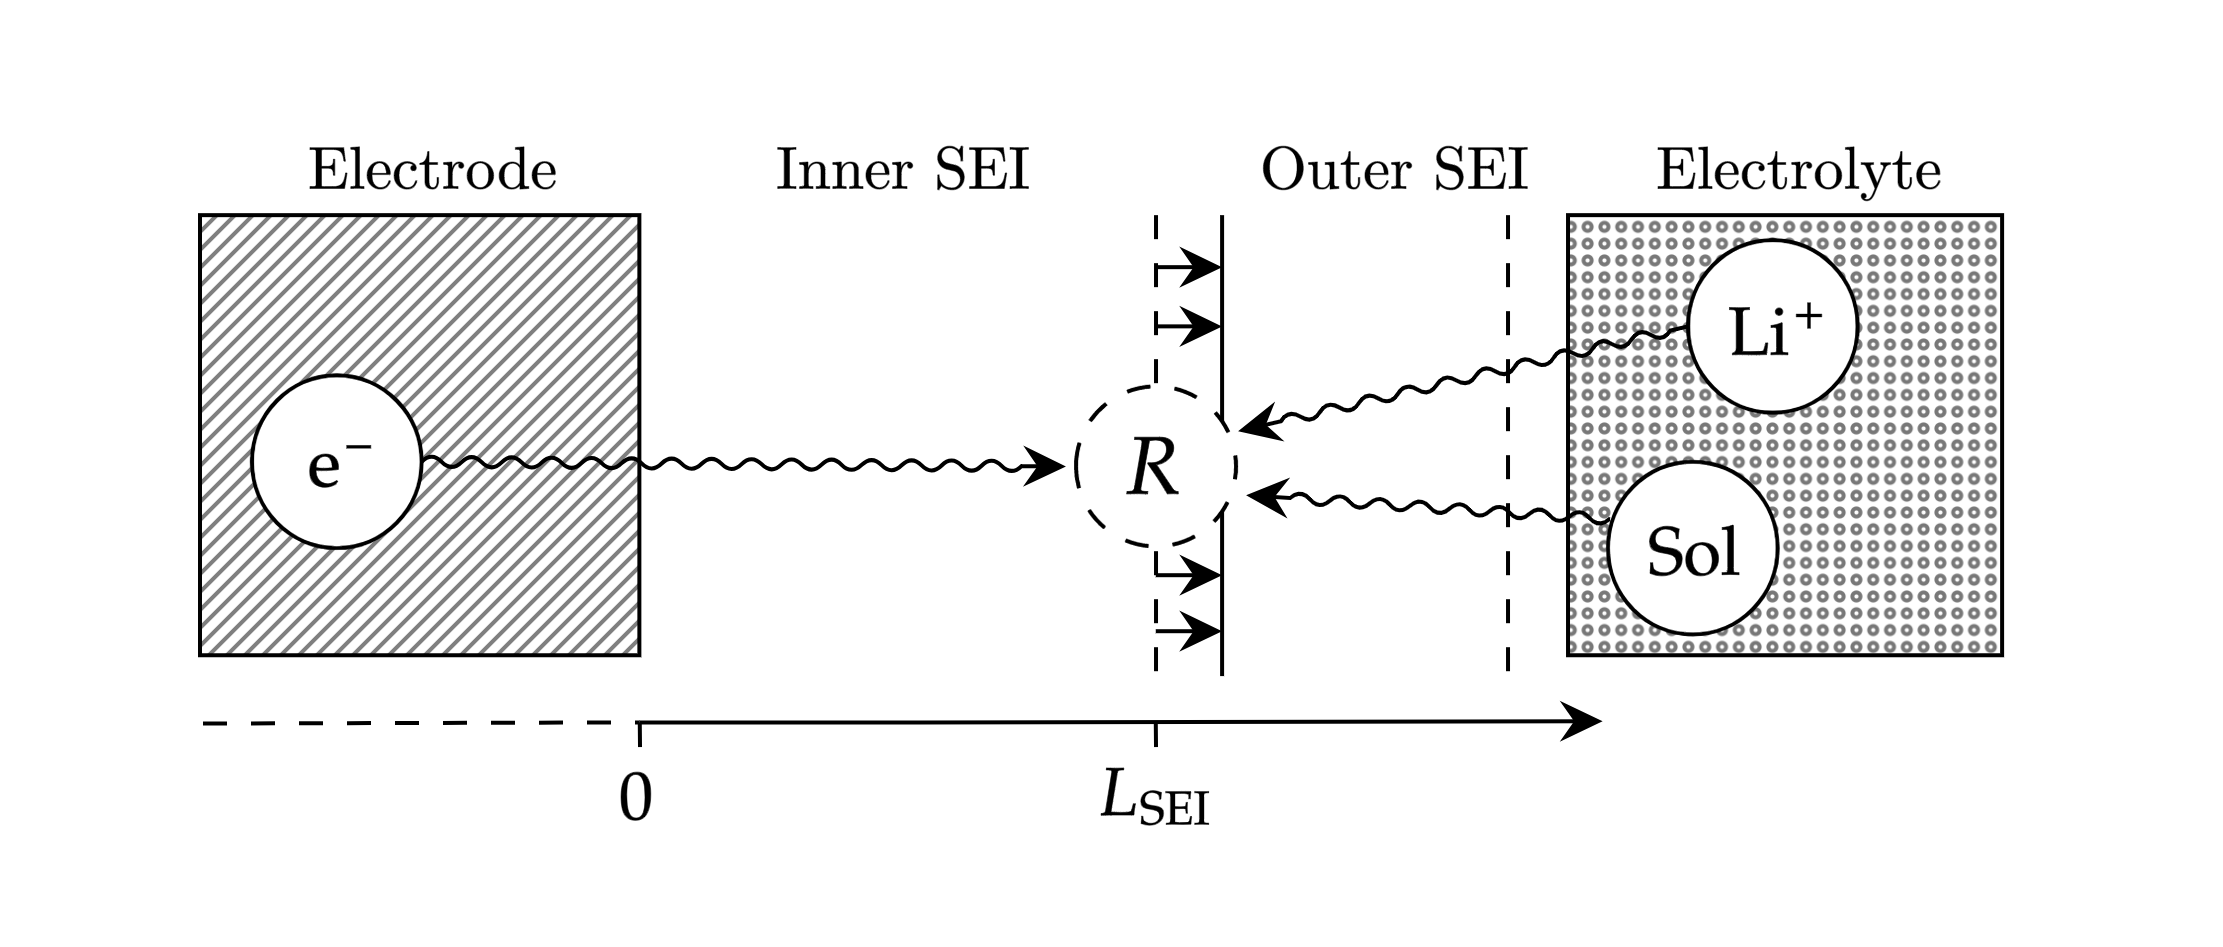
\includegraphics[width=\textwidth]{sei.png}
	\caption{Schematic of the SEI. The site of the SEI growth reaction is indicated by $R$, and the species involved in this reaction are indicated. Here, Sol refers to solvent molecules.}
	\label{fig:sei}
\end{figure}


\subsection{Glossary of terms}

\begin{infommitemize}
	\litem{Degradation} The deterioration of the cell usually in the form of capacity fade or reduced efficiency caused by rising internal resistances.
	\litem{Active material} The material in the electrode within which lithium can be intercalated is known as the active material.
	\litem{Binder material} The binder is a porous polymer matrix that ``binds'' the active material together and conducts electrons. This ensures electrical contact between the active material and current collector is maintained.
	\litem{Current collector} A sheet of aluminium or copper foil that provides a pathway from the tabs and external circuit to the electrodes.
	\litem{Electrode} An electrically conducting material consisting of active material and binder.
	\litem{Electrolyte} An ionically conducting material consisting of positively and negatively charged ionic species within a neutral solvent.
	\litem{Intercalation} The process in which an atom is inserted into a layered material such as graphite.
	\litem{Asymptotic Methods} A set of mathematical methods for describing the behaviour of a system in a particular limit (e.g. as a parameter tends to zero). These methods can be used to gain good approximate solutions when certain parameters are either large or small.
	\litem{State of Charge (SoC)} How charged the cell is. If SoC is 1 then the cell is fully charged. If SoC is 0 then the cell is fully discharged.
\end{infommitemize}

\newpage
\subsection{Project aims}
\infommmarginnote{We aim to develop efficient models of lithium-ion batteries and SEI growth.}
The degradation of lithium-ion batteries is highly complex with many little-understood mechanisms occurring simultaneously. To fully understand the effects of these mechanisms, they must be incorporated into a model of a full lithium-ion pouch cell. Since degradation occurs over many cycles and over very long time periods, it is essential to first develop mathematical models of pouch cells which can efficiently simulate long-term effects. Once this framework is in place, in-depth analysis of the individual degradation mechanisms should be performed and the resulting models incorporated into the efficient full cell models. Here, we shall focus on one of the key degradation mechanisms, the growth of the SEI. Therefore, the two key aims of this project are
\begin{infommitemize}
	\item Develop efficient mathematical models of a full lithium-ion pouch cell
	\item Develop a mathematical model of SEI growth
\end{infommitemize}

\section{Efficient models of a Lithium-ion pouch cell}

\subsection{Mathematical modelling}
\infommmarginnote{We first develop a detailed physics-based model of a lithium-ion battery.}
We develop a full three-dimensional mathematical model of a lithium-ion pouch cell as follows. To model the flow of electrons in the current collectors and electrodes, we enforce conservation of charge and employ Ohm's law. In the active material particles, we consider conservation of mass and assume lithium is transported down gradients in lithium. In the electrolyte, we enforce the conservation of mass for both the positive and negative ionic species. The electrochemical reactions are modelled using the phenomenological Butler--Volmer relations. Finally, we account for thermal effects by employing an energy conservation equation and accounting for Ohmic and reaction heat sources.

\begin{figure}[h]
	\centering
	\begin{overpic}[width=0.7\textwidth]{grid2.png}
		\put(12, 67){2+1D DFN}
		\put(38, 67){2+1D SPMe}
		\put(62, 67){2+1D SPM}

		\put(14, 34){DFNCC}
		\put(39, 34){SPMeCC}
		\put(64, 34){SPMCC}

		\put(16, 2){DFN}
		\put(41, 2){SPMe}
		\put(66, 2){SPM}
	\end{overpic}
	\caption{Pictorial representation of derived suite of reduced-order models of a lithium-ion pouch cell.}
	\label{fig:suite}
\end{figure}

\infommmarginnote[-6.5em]{We use asymptotic methods to simplify this model taking into account the cell geometry and the timescales of key physical processes within the cell.}
This model is very detailed and too computationally expensive for the study of long-term degradation. We therefore adopt \emph{asymptotic methods} to systematically simplify this model. There are two key parameters that we take advantage of to simplify the model. The first is the \emph{aspect ratio} of the cell, that is the cell is much taller and wider than it is thick (in the through-cell direction). The second parameter is the ratio of the typical timescale for diffusion in the electrolyte to the typical discharge time. Typically the discharge timescale is around an hour whereas the electrolyte diffusion timescale is only around a minute. By considering different combinations of asymptotic limits of these two parameters, we develop the suite of reduced-order models of a lithium-ion pouch cell presented in \Cref{fig:suite}.

\infommmarginnote[1.5cm]{Different combinations of asymptotic simplifications give rise to different simplified models.}
\Cref{fig:suite} can be understood as follows. In the top left, we present the most complex reduced model that is derived from an asymptotic limit in the aspect ratio. Instead of a full three-dimensional cell model, this model consists of two-dimensional models for the current collectors coupled to a detailed one-dimensional through-cell model at every point. By proceeding downward in \Cref{fig:suite}, we take further advantage of the aspect ratio. In the bottom left, the current collectors behave uniformly and the model is reduced to a single one-dimensional through-cell model. In the middle row on the left, an ``in-between'' model is developed which accounts for some of the higher dimensional effects but maintains much of the simplicity of the one-dimensional model. Proceeding from left to right, simplifications are made by taking advantage of the ratio of the electrolyte diffusion and discharge timescales. In the top right, all the active material particles behave in the same way and so only one representative particle must be solved for in each electrode. At the top of the middle column, and `in-between' model is developed that accounts for some of the more complex effects in the through-cell direction but maintains much of the computational simplicity of the model in the top right. The other models are then different combinations of these two sets of simplifications.

\subsection{Results}
We first compared the predictions of key output variables that our asymptotically reduced models make with those of ad-hoc reduced models of similar complexity from literature. The results for the SPMe model (middle column, bottom row of \Cref{fig:suite}) are presented in \Cref{fig:errors}. We found that our models outperform those in the literature in terms of accuracy and are equivalent in terms of computational time across all operating currents. Following these results, we identified the terms in the ad-hoc models that gave rise to greater errors.
\infommmarginnote[1.8cm]{Our simplified models perform better than others from the literature.}
\begin{figure}[h]
	\centering
	\begin{overpic}[width=\textwidth]{ad-hoc-spme.png}
		\put(82.5, 35.5){Asymptotic}
		\put(82.5, 32.2){Literature 1}
		\put(82.5, 28.8){Literature 2}
		\put(82.5, 25.5){Literature 3}
	\end{overpic}
	\caption{Voltage errors of asymptotic SPMe and similar models from the literature at different currents. Here, C is this C-rate which is the current that fully discharges the battery in one hour.}
	\label{fig:errors}
\end{figure}

We also conducted a full numerical comparison of each of the models in \Cref{fig:suite} and condensed these results into a single table. A simplified version of this table is presented in \Cref{tab:summary-table}. This table presents the solve speed, memory requirements, and the accuracy of its prediction of key internal cell variables such as electric potentials, lithium concentrations, cell temperature, and cell voltage. This table allows one to select a model of appropriate fidelity for a particular application. In particular, we identify the SPMeCC as a fast model, with low memory requirements, and a moderate performance at recovering the key cell variables required as inputs in studies of degradation. Therefore, the SPMeCC is a good model to adopt for studying the degradation of lithium-ion batteries.

\begin{table}[h]
    \centering
	\resizebox{\textwidth}{!}{%
    \begin{tabular}{l | c c | c c c | c c c}\toprule
         \multirow{2}{4em}{Model} & \multirow{2}{4.8em}{Solve time}  & \multirow{2}{4em}{Memory} & \multicolumn{3}{c|}{$I=\SI{1}{C}$} &  \multicolumn{3}{c}{Voltage} \\
         & & & Potential & Concentration & Temperature & $I<\SI{1}{C}$ & $\SI{1}{C}<I<\SI{4}{C}$& $I>4C$ \\ \midrule
         2+1D DFN & \xmark & \xmark & \cmark & \cmark & \cmark & \cmark & \cmark & \best \\
         2+1D SPMe & \xmark & \okmark & \cmark & \cmark & \okmark & \okmark & \okmark & \xmark \\
         2+1D SPM & \okmark & \okmark & \okmark & \okmark & \xmark & \okmark & \xmark & \xmark \\
         DFNCC & \okmark & \okmark & \okmark & \xmark & \cmark & \cmark & \cmark & \cmark \\
         SPMeCC & \cmark & \cmark & \okmark & \xmark & \okmark  & \okmark & \okmark & \xmark \\
         SPMCC & \cmark & \cmark & \okmark & \xmark & \xmark & \okmark & \xmark & \xmark \\
         DFN & \okmark & \okmark & \xmark & \xmark & \xmark & \cmark & \cmark  & \cmark \\
         SPMe & \cmark & \cmark  & \xmark & \xmark & \xmark  & \okmark & \okmark & \xmark  \\
         SPM & \cmark & \cmark  & \xmark & \xmark & \xmark & \okmark & \xmark & \xmark \\ \bottomrule
    \end{tabular}
    }
    \caption{Simplified table comparing the models in \Cref{fig:suite}. Green is used to indicate faster/low memory/more accurate models and red to indicate slower/high memory/less accurate models. Orange indicates moderately performing models.}
    \label{tab:summary-table}
\end{table}

\newpage

\infommmarginnote[-5cm]{We provide a simplified model recommendation subject to user requirements.}
\subsection{Comments}
\begin{infommitemize}
	\item Developed a detailed model of a lithium-ion pouch cell
	\item Employed asymptotic methods to derive a suite of reduced-order models from this detailed model
	\item Provided a full numerical comparison and recommendation of appropriate fidelity model for studying degradation.
\end{infommitemize}

\section{Mathematical Modelling of the SEI}
\subsection{Mathematical Analysis}
\infommmarginnote{We developed a detailed model of the SEI.}
Within the inner SEI we considered the transport of species: lithium-ions and electrons. For each species, we enforced conservation of mass and took each species to be driven down gradients in concentration and also to be driven by gradients in the electric potentials because the species are both electrically charged. We then employed the phenomenological Butler--Volmer relations to model the reactions occurring on the interface between the active material and inner SEI as well as the reactions occurring on the interface between the inner SEI and outer SEI.

\infommmarginnote{We simplified this model by employing asympotic methods and found excellent agreement between the full and simple models.}
This model is too detailed to be incorporated into a model of a full lithium-ion cell and also contains a large number of unknown parameters. To simplify this model, we again employed asymptotic methods. In this case, we considered a limit in which the timescale for the diffusion of electrons through the SEI was long relative to the timescales of the reactions involving electrons. We also took the limit in which the timescale of lithium intercalation reaction at the active material--inner SEI interface was long compared to the timescale for the diffusion of lithium-ions through the inner SEI and the timescale of the reaction at the inner SEI--outer SEI interface. We compared this simplified model with the full model and found excellent agreement between the two for appropriate parameter values.

\subsection{Results}
We took our simplified SEI model and compared it with experimental capacity fade data. In the experiment lithium-ion cells were stored at different \emph{States-of-charge} (SoC) and temperatures. The capacity of the cells were then checked after 1.9 months, 3.8 months, 6.5 months, and 9.5 month. Firstly, at lower SoC, we expect that additional degradations cause capacity fade in the lithium-ion cell. However, for SoC greater than 0.2, we observe excellent agreement between our model and the experimental data. In particular, our model captures well the temperature, SoC, and temporal dependence of capacity fade.

\begin{figure}[h]
	\centering
	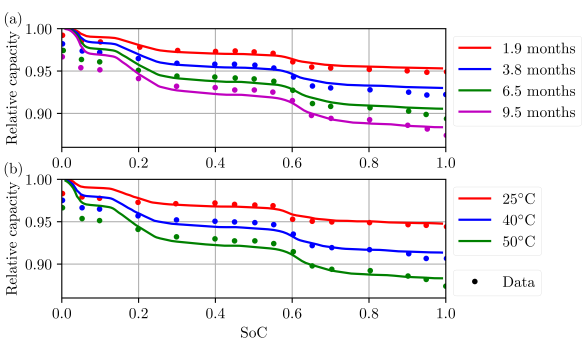
\includegraphics[width=\textwidth]{experimental-fit.png}
	\caption{Comparison of SEI model with experimental capacity fade data. Two parameters in our SEI model were treated as adjustable parameters: (a) time dependence at $\SI{50}{\celsius}$; (b) temperature dependence after 9.5 months.}
	\label{fig:sei}
\end{figure}

After validating our SEI model against experimental data, we incorporated into the SPM, the simplest of the full cell models in \Cref{fig:suite}. We studied then used this model to study SEI growth under dynamic loads. From this study, we developed a map of `safe' and `dangerous' operating conditions for degradation. This map is presented in \Cref{fig:degradation-map}. We observe that degradation occurs most at high SoCs and during charging of a cell and least at low SoCs and during a discharge.
\infommmarginnote[-8cm]{Our simple SEI model captures the temperature, SoC, and temporal dependence of capacity fade.}

\infommmarginnote[2cm]{We provided a map of SEI growth across different operating conditions.}
\begin{figure}[h]
	\centering
	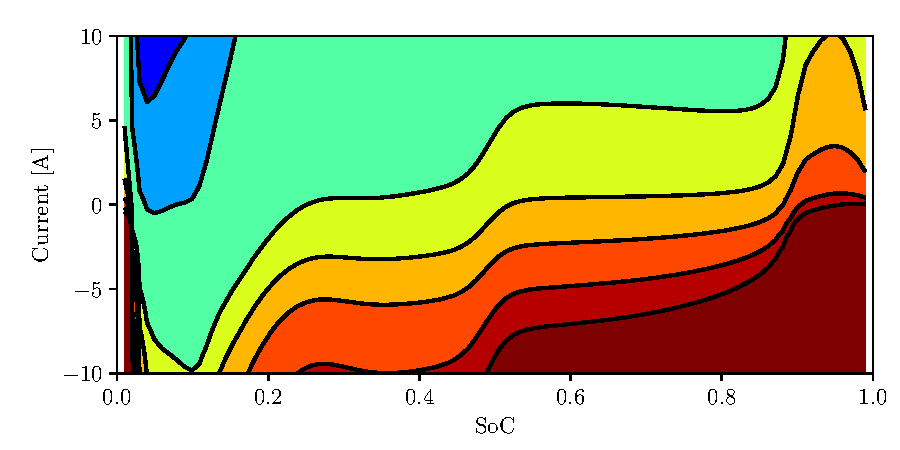
\includegraphics[width=0.9\textwidth]{map.pdf}
	\caption{Map of `safe' and `dangerous' operating conditions for degradation. Red indicates high degradation, and blue indicates low degradation. A ositive current corresponds to discharging the cell.}
	\label{fig:degradation-map}
\end{figure}


\subsection{Comments}
\begin{infommitemize}
	\item Developed a detailed model of SEI and used asymptotic methods to simplify this model.
	\item Found excellent agreement between SEI model and experimental capacity fade data.
	\item Incorporated SEI model into a model of a full lithium-ion cell and determined `safe' and `dangerous' operating conditions for degradation.
\end{infommitemize}

\newpage
\section{Discussion, conclusions \& recommendations}
We have tackled the problem of degradation in lithium-ion batteries by addressing two key challenges:
\begin{itemize}
	\item Develop efficient mathematical models of full lithium-ion cells.
	\item Develop an accurate model of SEI growth.
\end{itemize}
\infommmarginnote[-1em]{The SPMeCC is a good model of a lithium-ion cell for studying degradation.}
For the first challenge, we developed a detailed mathematical model of a full lithium-ion pouch cell and then used asymptotic methods to develop a suite of simplified models. We found that our models outperformed those of similar complexity in the literature. We also performed a full numerical comparison of all of these models and found that the SPMeCC is a good choice of model for studying degradation.

\infommmarginnote[2em]{SEI growth is worst at high SoC and during charging.}
For the second challenge, we developed a detailed model of SEI growth and then employed asymptotic methods to develop a simplified model that agreed well with the detailed model. We then compared this simple model with experimental capacity fade data and found excellent agreement. After validating this model, we then incorporated into a full model of a lithium-ion cell and developed a map of operating conditions and their relative rates of degradation. We found that the highest rates of degradation occur during charging and a low SoCs.


\section{Potential Impact}
\infommmarginnote{All models have been implemented in an easy-to-use software package for Siemens to use. \\[1em]
Models can be used to efficiently simulate degradation due to SEI growth and can be easily extended to account for other mechanisms.
}
All of the models developed during this project have been implemented within an open-source easy-to-use battery modelling package called PyBaMM (Python Battery Mathematical Modelling). Coupled with the model comparisons in \Cref{tab:summary-table}, this provides an excellent resource for other battery researchers and Siemens to employ. Further, the models have all been implemented in a modular fashion so that additional degradation mechanisms can be easily incorporated into the framework removing duplicate work across institutions and accelerating battery modelling research in general. Siemens are planning to interface PyBaMM with internal software to take advantage of the modular framework and efficient mathematical models developed during this project.

Ian Wilkinson, Programme Manager at Siemens said: ``\emph{Scott's work applying advanced mathematical techniques to the modelling of lithium-ion batteries has proved very successful. The suite of efficient mathematical models of lithium-ion cells that Scott has developed dramatically cuts down computation time in studying degradation whilst retaining accuracy. By implementing his work within PyBaMM, he has made it easily accessible to others, which is helping accelerate research in this area. Siemens is also looking into interfacing PyBaMM with its own computational software to leverage the benefits of Scott's work.}''

% Add the bibliography.
% \begin{small}
%	\nocite{*} % Publishes any unused references.
% \bibliography{references}
% \end{small}

\clearpage
\end{document}
